\section{Technical Appendix}
\label{sec:appendix}

\subsection{Quality Criterion and Break-Even Derivation}
\label{sec:appendix-break-even}

The cost comparison applies subject to a user-specified quality tolerance.
Let $\mathrm{Perf}_{\mathrm{PCU}}$ and $\mathrm{Perf}_{\mathrm{LESS}}$ denote
the two selectors' downstream scores. We treat them as tied in quality when
\begin{equation}
  \Delta_{\mathrm{quality}}=\mathrm{Perf}_{\mathrm{PCU}}-\mathrm{Perf}_{\mathrm{LESS}},
  \qquad \lvert\Delta_{\mathrm{quality}}\rvert\le\epsilon.
  \label{eq:quality-tie}
\end{equation}
Here $\epsilon$ is the largest acceptable absolute difference.

Let $P$ and $Q$ denote the numbers of PEFT configurations and tasks,
respectively. PCU-Select is cheaper when its shared offline cost plus its $PQ$
online-selection costs falls below LESS's $P$ datastore-construction costs plus
its $PQ$ ranking costs. Solving this inequality gives
\begin{equation}
  P > P^{\star}=
  \frac{C_{\mathrm{offline}}}
  {C^{\mathrm{data}}_{\mathrm{LESS}}+
  Q(C^{\mathrm{rank}}_{\mathrm{LESS}}-C^{\mathrm{pair}}_{\mathrm{PCU}})},
  \label{eq:break-even}
\end{equation}
provided that the denominator is positive. For $Q=4$, PCU-Select's measured
online cost is 1.51 GPU-hours per configuration, or
$C^{\mathrm{pair}}_{\mathrm{PCU}}=1.51/4=0.3775$ GPU-hours per PEFT--task pair
(displayed as 0.38 in the tables). LESS costs 63.2 GPU-hours per four-task
configuration, while PCU-Select pays 144.0 GPU-hours offline plus 1.51
GPU-hours per configuration. Therefore,
\begin{equation}
  P^{\star}=\frac{144.0}{63.2-1.51}=2.33.
  \label{eq:break-even-measured}
\end{equation}
Because $P$ is integer-valued, PCU-Select costs less at $P\ge3$. If all four
task pairs additionally use 500 reduced calibration labels, the marginal cost
becomes $1.51+4(1.05)=5.71$ GPU-hours and
$P^{\star}=144.0/(63.2-5.71)=2.50$; the integer break-even point remains three
configurations.

\subsection{Per-Task Results Behind the Main Table}
\label{sec:appendix-per-task}

Table~1 in the main paper summarizes four task-native percentage scores: GSM8K
exact match, HumanEval Pass@1, MMLU accuracy, and TyDiQA F1. Because these
metrics have different scales, ceilings, and seed variances, their average can
hide task-level differences. Table~\ref{tab:per-task-compact} therefore reports
them separately. For a baseline $b$, we define
$\Delta b=\mathrm{Perf}_{\mathrm{PCU}}-\mathrm{Perf}_{b}$, so positive values
favor PCU-Select. Each PEFT cell is first averaged over the three
target-training seeds; the task-level value then averages the five seen PEFT
configurations. For LESS, the table also reports a descriptive 95\% interval
obtained by resampling the five paired PEFT-level differences. Parentheses give
the number of configurations for which PCU-Select has the higher seed-averaged
score.

PCU-Select has a higher PEFT-averaged score than RDS+ and Influence on each of
the four tasks. Its comparison with LESS varies by task: the paired
PCU-Select-minus-LESS interval is positive on MMLU ($+0.67$ Acc,
$[+0.24,+1.08]$), crosses zero on GSM8K ($+0.29$ EM,
$[-0.04,+0.58]$) and HumanEval ($-0.04$ Pass@1, $[-0.44,+0.31]$), and is
negative on TyDiQA ($-0.77$ F1, $[-1.18,-0.43]$). These opposing task-level
differences yield the registry-level mean gap of $+0.04$ points reported in the
main paper. The observed registry-average performance is therefore close, but
the task-level results are heterogeneous.

\begin{table*}[t]
\centering
\small
\setlength{\tabcolsep}{5pt}
\begin{tabular}{llrrrr}
\toprule
Task & Metric & PCU & $\Delta$RDS+ & $\Delta$Inf. & $\Delta$LESS (95\% CI) \\
\midrule
GSM8K & EM & 22.20 & +0.55 (5/5) & +0.58 (5/5) & $+0.29$ $[-0.04, +0.58]$ (4/5) \\
HumanEval & Pass@1 & 17.06 & +0.64 (4/5) & +0.24 (4/5) & $-0.04$ $[-0.44, +0.31]$ (2/5) \\
MMLU & Acc & 49.14 & +1.55 (5/5) & +1.00 (5/5) & $+0.67$ $[+0.24, +1.08]$ (4/5) \\
TyDiQA & F1 & 52.30 & +0.22 (3/5) & +0.17 (4/5) & $-0.77$ $[-1.18, -0.43]$ (0/5) \\
\bottomrule
\end{tabular}
\caption{Task-level summary of the main 10\% budget result. Values are averaged over the five seen PEFT configurations. $\Delta$RDS+ and $\Delta$Inf. are absolute native-point gains over PEFT-agnostic baselines; $\Delta$LESS is the paired difference against per-PEFT LESS with a descriptive 95\% cell-resampling interval over PEFT cells. Parentheses report PCU-Select wins among the five PEFT cells for each task; column totals are 17/20, 18/20, and 10/20, respectively.}
\label{tab:per-task-compact}
\end{table*}


\paragraph{Task- and configuration-level differences.}
The largest task-aggregated deficit to LESS occurs on TyDiQA, where PCU-Select
is lower by $0.77$ F1. The largest configuration-aggregated deficit occurs for
MLP-only LoRA (L-r8-mlp), at $0.57$ points. Under this configuration,
PCU-Select's HumanEval and TyDiQA results have downstream-seed SDs of $0.68$
and $0.62$, respectively. These SDs quantify variation across target-training
seeds, not uncertainty predicted by the scorer. The results thus localize the
largest observed discrepancies to TyDiQA and L-r8-mlp, but do not by themselves
identify a causal mechanism.

\subsection{Evaluation Protocols}
\label{sec:appendix-protocols}

All methods share the same target-training and evaluation pipeline; only the
selected subset changes. Target training uses the Llama-2-7B
backbone~\cite{touvron2023llama2}, freezes the backbone, and trains only the
target PEFT. Table~\ref{tab:appendix-peft-registry} lists the per-configuration
learning rates (2e-4 for LoRA, 5e-4 for (IA)$^3$, 3e-4 for adapters, and 1e-4
for L-r64-all). The fixed recipe uses AdamW and a cosine schedule with a $0.03$
warmup ratio. It runs for $1000$ steps with
bfloat16, gradient clipping at $1.0$, and maximum sequence length $1024$. A
per-device batch of $16$ over $8$ GPUs gives a global batch of $128$.

At the 10\% budget, the selected subset holds $30$K examples. The $1000$ steps
therefore process $128$K samples, or about $4.3$ passes over the subset. The
dataloader shuffles the full subset each epoch, so it uses every selected example.
Selected instructions average $\approx512$ tokens, and length-bucketed batches
reduce padding.

With FlashAttention-2~\cite{dao2024flashattention2} and gradient checkpointing,
each step takes approximately $5.8$ wall-clock seconds. At the observed mean
sequence length, this corresponds to about $22$ samples/s in aggregate and
$1.4$K tokens/s per GPU. A 1000-step run takes approximately $96$ minutes, or
$12.8$ GPU-hours under the
$(\text{wall seconds}\times\text{GPU count})/3600$ convention. Because all
selectors use the same target-training recipe and step budget, we exclude
target training from the selection-stage cost comparison.

The primary downstream metric for each task is its standard task-native score,
computed by a task evaluator injected into the training runner. We log
held-out response-LM loss as an auxiliary diagnostic (\texttt{eval\_loss}) but use
only the primary task metric for comparison. Concrete per-task decoding and
scoring protocols are:

\begin{itemize}
  \item \textbf{GSM8K (exact match).} Chain-of-thought generation~\cite{cobbe2021gsm8k} with greedy
    decoding; the evaluator extracts the final numeric answer and checks exact
    match.
  \item \textbf{HumanEval (Pass@1).} The standard unbiased Pass@1 estimator~\cite{chen2021humaneval}:
    sampling at temperature $0.2$ with $n{=}20$ samples per problem, scored by
    unit-test execution. This is a multi-sample estimate of Pass@1, not a single
    greedy sample.
  \item \textbf{MMLU (accuracy).} Log-likelihood scoring~\cite{hendrycks2021mmlu} of the four answer
    options; the evaluator selects the highest-likelihood option without
    free-form generation.
  \item \textbf{TyDiQA-GoldP (F1).} Greedy decoding of the answer span~\cite{clark2020tydiqa}, scored
    with token-level F1 against the gold answers.
\end{itemize}

An evaluation adapter supplies these task-specific evaluators to the runner
through the \texttt{-{}-task-metric-factory} hook. We use the same fixed decoding
and scoring settings for every selector; they define the metrics in this study
and need not match every public evaluation harness.

Under our evaluation pipeline, untuned Llama-2-7B~\cite{touvron2023llama2}
scores $13.9$ on GSM8K, $12.4$ on HumanEval, $43.9$ on MMLU, and $46.2$ on
TyDiQA. Our MMLU value is not directly comparable with Meta's reported $45.3$
because the prompt and evaluation harness differ. Every selector-trained model,
including Random, exceeds the corresponding untuned score on all four tasks.
Random therefore serves as the reference for gains beyond uniform subset
selection.

\subsection{Reproducibility Supplement}
\label{sec:appendix-repro}

This section records the implementation details needed to reproduce the
reported experiments. It pins the public releases and states the
experiment-specific conversion, sampling, and evaluation rules explicitly.

\paragraph{Data provenance and deduplication.}
The candidate pool holds 300K mixed instruction examples drawn from seven public
instruction corpora. Table~\ref{tab:appendix-provenance} identifies the public
snapshot, split, record conversion, and final contribution of every source.

\begin{table*}[t]
\centering
\small
\setlength{\tabcolsep}{3pt}
\begin{tabular}{@{}>{\raggedright\arraybackslash}p{.17\textwidth}
                    >{\raggedright\arraybackslash}p{.29\textwidth}
                    >{\raggedright\arraybackslash}p{.38\textwidth}r@{}}
\toprule
Source & Public release used & Conversion to an instruction--response record & Final rows \\
\midrule
FLAN v2~\cite{longpre2023flan} & \texttt{Open-Orca/FLAN}, third-party FLAN 2022
  materialization, rev.\ \texttt{6845b1b3}, train partitions & Published
  \texttt{inputs} $\rightarrow$ instruction and \texttt{targets}
  $\rightarrow$ response; stratify by component task & 110{,}000 \\
OpenOrca~\cite{lian2023openorca} & \texttt{Open-Orca/OpenOrca}, default/train,
  rev.\ \texttt{aaeb6859} & Concatenate nonempty \texttt{system\_prompt} and
  \texttt{question}; use \texttt{response} as the target; stratify across the
  released GPT-4 and GPT-3.5 partitions & 70{,}000 \\
Tulu v2 SFT mix~\cite{ivison2023camels} &
  \texttt{allenai/}\allowbreak\texttt{tulu-v2-sft-mixture}, default/train,
  rev.\ \texttt{0bc269ee} & Retain alternating user/assistant messages and
  serialize the preceding turns as the instruction; stratify by the released
  \texttt{dataset} field & 50{,}000 \\
OASST1~\cite{kopf2023openassistant} & \texttt{OpenAssistant/oasst1},
  2023-04-12 release, default/train, rev.\ \texttt{fdf72ae0} & Reconstruct
  English conversation trees and pair each prompter turn with its highest-ranked
  positively reviewed assistant child & 30{,}000 \\
CodeAlpaca 20K~\cite{chaudhary2023codealpaca} &
  \texttt{sahil2801/CodeAlpaca-20k}, rev.\ \texttt{152bb5e9}, all 20{,}022
  source rows & Concatenate \texttt{instruction} and nonempty \texttt{input};
  use \texttt{output} as the response & 20{,}000 \\
Dolly 15K~\cite{conover2023dolly} &
  \texttt{databricks/}\allowbreak\texttt{databricks-dolly-15k} v1.0, train,
  rev.\ \texttt{bdd27f4d} & Concatenate \texttt{instruction} and nonempty
  \texttt{context}; use \texttt{response} as the target & 15{,}000 \\
WizardLM Evol-Instruct 70K~\cite{xu2024wizardlm} &
  \texttt{WizardLMTeam/}\allowbreak\texttt{WizardLM\_evol\_}%
  \allowbreak\texttt{instruct\_70k}, train,
  rev.\ \texttt{16b48bd8} & Use \texttt{instruction} as the prompt and
  \texttt{output} as the response & 5{,}000 \\
\midrule
Total & & & 300{,}000 \\
\bottomrule
\end{tabular}
\caption{Candidate-pool provenance, pinned public releases, and record
construction. Revision strings are eight-character prefixes of the public
repository commits. Counts are final post-filter contributions.}
\label{tab:appendix-provenance}
\end{table*}

We apply one sampling rule to all seven releases. Within each source, a PCG64
generator with seed 0 shuffles source-native IDs (or original row indices when
no ID is provided). We scan this order until the source reaches its target
quota. FLAN v2, Tulu v2, and OpenOrca preserve the proportions of their eligible
rows across FLAN component tasks, Tulu's \texttt{dataset} field, and OpenOrca's
GPT-4/GPT-3.5 partitions, respectively. Largest-remainder rounding converts
these proportions to integer stratum quotas. Rejected or duplicate records are
replaced by later records from the same source and stratum, so both source and
stratum totals remain fixed. We preserve the upstream source ID with every
retained record.

Deduplication then runs in three stages. First, it removes exact duplicates by
the content hash of the normalized instruction--response pair. Second, it
removes normalized-string matches after lowercasing and stripping whitespace and
punctuation. Third, MinHash LSH removes near-duplicates using 128 permutations
and a Jaccard threshold of $0.8$. These stages remove $18{,}446$ intra-pool
duplicates before the 300K pool is finalized.

Licensing follows the pinned public releases. The OpenOrca and WizardLM dataset
cards record MIT, although upstream terms may also apply. OASST1 uses
Apache-2.0, CodeAlpaca uses CC-BY-NC-4.0, and Dolly uses CC-BY-SA-3.0. FLAN
components retain their component-specific licenses. The Tulu v2 wrapper is
distributed under ODC-BY-1.0, while its constituent sources retain their own
terms. We use all non-commercial or mixed-license components only for
non-commercial research.

\paragraph{Benchmark decontamination.}
We decontaminate the pool against the test items of GSM8K, HumanEval, MMLU, and
TyDiQA. The filter checks exact matches, normalized-string matches, $13$-gram
overlap, and MinHash LSH near-duplicates. The $13$-gram stage removes candidates
with Jaccard overlap of at least $0.5$; the MinHash stage uses a threshold of
$0.8$. The filter removes $1{,}742$ pre-finalization candidates ($0.58\%$ of the
pool size). We then backfill from the same source buckets to keep the final pool
at 300K examples, so Table~\ref{tab:appendix-provenance} reports final
post-filter counts. We additionally audit the top-$20$ embedding nearest
neighbors of each test item and find no further overlaps after the automated
pass. All reported results are on the decontaminated pool.

\paragraph{Task sketch construction and HumanEval.}
Each task sketch contains 32 examples drawn with fixed seed 0 and stratified by
response length. For GSM8K, MMLU, and TyDiQA, we sort the eligible training or
development records by response character count, split them into three equal
index ranges, and use Python's \texttt{random.Random(0)} to draw 11, 11, and 10
examples from the short, medium, and long ranges. Every sketch remains disjoint
from its task's evaluation split.

HumanEval has no official training or development split. Its sketch is therefore
source-balanced: 16 examples come from the \texttt{full}/\texttt{train} split
(374 rows) of MBPP~\cite{austin2021program}, public revision
\texttt{4bb6404f}, and 16 come from the CodeAlpaca 20K release pinned in
Table~\ref{tab:appendix-provenance}. For MBPP, \texttt{text} is the instruction
and the canonical \texttt{code} solution is the response; the tests are retained
for decontamination and auditing but are not appended to either field. Within
each source, we filter against the 164 HumanEval evaluation problems, form
response-character-length terciles, and use \texttt{random.Random(0)} to draw 6,
5, and 5 examples from the short, medium, and long terciles, respectively. Exact
content matching and AST-normalized function-signature matching are applied
before sampling.

Because the candidate pool also contains CodeAlpaca, we test all 32 sketch items
against the pool and exclude every content-hash or AST-signature match before
selection; the CodeAlpaca quota is then refilled from its seeded order. Thus the
sketch is disjoint from both the HumanEval evaluation set and the candidate
pool. We enforce the same disjointness for every selector because the sketch is
the shared selection signal.

\paragraph{PEFT registry.}
Table~\ref{tab:appendix-peft-registry} lists all 17 PEFT configurations:
five seen, nine unseen same-family configurations, and three unseen families.
The unseen-configuration transfer study evaluates eight held-out
targets---L-r32-qkvo, AD-b16, L-r64-all, AD-b256, L-r8-highlayers, PRE-l16,
PT-l32, and LN---while the configuration-sensitivity study uses the additional
LoRA variants. All use $1000$ steps, a cosine schedule, and $0.03$ warmup;
learning rates vary by configuration.
The LN configuration trains the \texttt{input\_layernorm} and
\texttt{post\_attention\_layernorm} scale parameters in every Transformer
block and excludes the final model-level RMSNorm.

\begin{table*}[t]
\centering
\small
\setlength{\tabcolsep}{4pt}
\begin{tabular}{@{}llllccl@{}}
\toprule
Config & Family & Target modules & Capacity & LoRA scaling & LR & Group \\
\midrule
L-r8-qv        & LoRA      & q, v                       & $r{=}8$   & 16  & 2e-4 & seen \\
L-r16-qkvo     & LoRA      & q, k, v, o                 & $r{=}16$  & 32  & 2e-4 & seen \\
L-r8-mlp       & LoRA      & up, down                   & $r{=}8$   & 16  & 2e-4 & seen \\
IA3-attnmlp    & IA$^3$    & k, v, down                 & --        & --  & 5e-4 & seen \\
AD-b64         & Adapter   & block-residual             & $b{=}64$  & --  & 3e-4 & seen \\
\midrule
L-r4-qv        & LoRA      & q, v                       & $r{=}4$   & 8   & 2e-4 & unseen-config \\
L-r32-qkvo     & LoRA      & q, k, v, o                 & $r{=}32$  & 64  & 2e-4 & unseen-config \\
L-r64-all      & LoRA      & q, k, v, o, up, down, gate & $r{=}64$  & 128 & 1e-4 & unseen-config \\
L-r8-lowlayers & LoRA      & q, v (low third)           & $r{=}8$   & 16  & 2e-4 & unseen-config \\
L-r8-highlayers& LoRA      & q, v (high third)          & $r{=}8$   & 16  & 2e-4 & unseen-config \\
L-r16-hlr      & LoRA      & q, k, v, o                 & $r{=}16$  & 32  & 5e-4 & unseen-config \\
AD-b16         & Adapter   & block-residual             & $b{=}16$  & --  & 3e-4 & unseen-config \\
AD-b256        & Adapter   & block-residual             & $b{=}256$ & --  & 3e-4 & unseen-config \\
IA3-attnonly   & IA$^3$    & k, v                       & --        & --  & 5e-4 & unseen-config \\
\midrule
PRE-l16        & Prefix    & attention                  & len${=}16$& --  & 2e-4 & ood-family \\
PT-l32         & P-Tuning  & attention                  & len${=}32$& --  & 2e-4 & ood-family \\
LN             & LN Tuning & input/post-attn RMSNorm    & 2 scales/layer & -- & 2e-4 & ood-family \\
\bottomrule
\end{tabular}
\caption{Full PEFT registry (all 17 configurations). ``LoRA scaling'' is the
LoRA $\alpha$ hyperparameter and is distinct from the intervention-site weight
$\tilde{w}_p^\omega$ defined in the main paper; it applies only to LoRA rows.
Adapters are single post-block residual bottlenecks (one per layer); IA$^3$
scales the listed activations. LN Tuning updates per-block RMSNorm scales~\cite{wang2022lntuning,touvron2023llama2}.
Learning rates for the three OOD-family targets
use the registry default (2e-4). Layer placement is all layers unless noted;
low/high-third placements use the bottom/top $\lceil n/3 \rceil$ layers of the
32-layer backbone.}
\label{tab:appendix-peft-registry}
\end{table*}

\paragraph{Intervention sites and gradient signatures.}
The site space $\Omega$ provides a shared coordinate system across PEFT families.
It contains $24$ sites: $8$ layers $\times\ 3$ module outputs per layer
(\texttt{attn\_out}, \texttt{mlp\_out}, and \texttt{block\_residual}). Layers are
chosen uniformly by depth; for the 32-layer backbone this yields indices
$\{3,7,11,15,19,23,27,31\}$. Each site carries a Johnson--Lindenstrauss random
projection~\cite{johnson1984jl} $\Phi_\omega \in \mathbb{R}^{256 \times 4096}$ with entries drawn
$\mathcal{N}(0, 1/256)$ under a per-site seed
$\mathrm{SHA256}(\texttt{site}, \texttt{global\_seed}{=}0)$; projected gradients
are $L_2$-normalized per row. Each sample's signature contains $24\times256$
values. In bfloat16, these projected gradients occupy approximately $3.69$~GB
($3.43$~GiB) for the 300K-example pool. They are stored as a memory-mapped array
and reused during offline proxy-label construction; online PCU-Select scoring
uses cached $z_x$ features rather than this gradient store. A configuration
activates sites through its mask and the capacity factor
$\kappa(p,\omega)=\tanh\!\big(\eta\log(1+\mathrm{cap}(p,\omega)/d_{\mathrm{model}})\big)$,
with $\eta{=}1.0$. Operator type enters the explicit PEFT code rather than a
scalar site prior; Table~\ref{tab:capacity} gives the family-specific capacity
mapping.

\paragraph{Conditional scorer.}
The conditional scorer estimates a sample's utility for a specific task and
PEFT configuration. It has three input towers: sample
$z_x \in \mathbb{R}^{848}$, PEFT condition $z_p \in \mathbb{R}^{128}$, and task
sketch $z_t \in \mathbb{R}^{848}$.
Each tower uses a LayerNorm--Linear--GELU--Linear--LayerNorm MLP. Let
$h_x,h_t\in\mathbb{R}^{256}$ and $h_p\in\mathbb{R}^{128}$ denote the three tower
outputs. The concatenated condition $[h_p;h_t]$ produces 256-dimensional FiLM
scale and shift vectors~\cite{perez2018film}, which modulate $h_x$. In parallel,
a bilinear layer maps $(h_x,h_p)$ to a 64-dimensional interaction vector. The
concatenated 320-dimensional representation passes through a
Linear--GELU head that maps it to 256 dimensions. Two linear output heads then
predict mean utility $\widehat{\mu}_{\phi}$ and an example-dependent uncertainty
scale $\widehat{\sigma}_{\phi}$; the latter uses softplus with a floor of
$10^{-3}$.

We use $\widehat{\sigma}_{\phi}$ as a ranking penalty.
On held-out labels, its predicted standard deviation tracks realized error with
a 10-bin expected calibration error of $0.043$. In the downstream ablation,
setting the uncertainty penalty to zero lowers the reported average by $0.28$
points (Table~\ref{tab:ablations}).

Training separates cheap proxy learning from expensive short-update supervision.
Phase A pretrains on the gradient proxy for $3$ epochs at lr $3\times10^{-4}$
with loss weights (rank, reg, proxy, unc) $=(0,0,1,0)$. Phase B jointly fine-tunes
for $2$ epochs at lr $10^{-4}$ with weights $(1.0, 0.3, 0.5, 0.2)$. Both phases
use AdamW, batch size $256$, and gradient clipping at $1.0$. The four losses are a
BPR-style pairwise ranking loss, a Huber regression loss against short-update
labels, a Huber proxy-distillation loss against the gradient-proxy labels, and a
Gaussian negative-log-likelihood uncertainty loss. We track ranking NDCG on a
held-out split of PEFT/task pairs that excludes two configurations and one task
from Phase B. We keep the Phase-B checkpoint with the best held-out NDCG. The
scorer uses no dropout.

\paragraph{Selection, clustering, and quotas.}
At application time, the scorer ranks each example by
$q = \mu - \lambda\,\sigma$ with uncertainty penalty $\lambda{=}0.2$. The
penalty favors examples with high predicted utility and lower uncertainty.
Ranking alone can concentrate the subset in a few semantic regions, so PCU-Select
adds cluster-level coverage. It applies MiniBatch
$k$-means~\cite{sculley2010minibatch} to the joint
embeddings. It uses $k = \max(50, \lfloor\sqrt{N}\rfloor)$, batch size $4096$,
$n_{\text{init}}{=}3$, and random state $0$. Adaptive quotas allocate budget $B$
across clusters by
$b_k = \mathrm{round}\!\big(B\, (v_k^+)^{\gamma}\, |C_k|^{1-\gamma} / Z\big)$ with
$\gamma{=}0.6$. Here $v_k$ is the mean conservative score $q$ among the top
10\% of examples in cluster $C_k$, $v_k^+=\max(v_k,0)$, and
$Z=\sum_j(v_j^+)^\gamma |C_j|^{1-\gamma}$. The algorithm distributes
remainders by descending weight and trims over-allocation from the
lowest-weight clusters.

Targets far from the seen registry can additionally calibrate the scorer with a
small label set. The calibrated mean is
$\widehat{\mu}_{\mathrm{cal}}=\widehat{\mu}_{\phi}
+W_{\mathrm{cal}}[z_x;z_p;z_t]+b_{\mathrm{cal}}$. We freeze the shared scorer
and fit only the zero-initialized residual parameters $W_{\mathrm{cal}}$ and
$b_{\mathrm{cal}}$ for 200 epochs at lr $5\times10^{-3}$ (Adam, MSE). These
deployment calibration labels $u^{\mathrm{hi}}_{\mathrm{cal}}$ are a reduced form of the
offline short-update labels $u^{\mathrm{hi}}$. They use only the warm anchor and
horizon $h{=}1$, rather than both anchors and both horizons. Each label therefore
costs one quarter of the full offline routine in
Eq.~\eqref{eq:uhi-offline}. An offline label costs
$84.0/10{,}000=0.0084$ GPU-hours, while a calibration label costs
$\approx0.0021$ GPU-hours. Budgets of 200 and 500 labels therefore cost $0.42$
and $1.05$ GPU-hours per PEFT--task pair. The full routine would cost about four
times more. We use $200$ or $500$
$u^{\mathrm{hi}}_{\mathrm{cal}}$ labels for the OOD study.

\paragraph{Structural support levels.}
The structural support levels determine whether a PEFT code that differs from
the training registry is evaluated zero-shot or with calibration. The reported
$z_p\in\mathbb{R}^{128}$ contains only the site/operator mask, capacity, and
recipe vectors. Prefix, P-Tuning, and LN Tuning use the same
deterministic encoding rules as the seen families; no centroid, learned family
lookup, or functional fingerprint enters the reported model. We fixed this
registry-relative taxonomy before evaluating the held-out targets. \textbf{L0}
contains near-support
same-family targets (L-r32-qkvo and AD-b16). \textbf{L1} contains farther
same-family shifts (L-r64-all, AD-b256, and L-r8-highlayers). \textbf{L2}
contains unseen families (PRE-l16, PT-l32, and LN). These levels define
registry-relative structural support. L1 and L2 targets use the reduced
calibration protocol described above; their results test whether a small
target-specific label set can repair a larger structural shift.

\begin{table}[t]
\centering
\small
\setlength{\tabcolsep}{3pt}
\begin{tabular}{@{}p{.18\columnwidth}p{.29\columnwidth}p{.45\columnwidth}@{}}
\toprule
Level & Definition & Evaluation mode \\
\midrule
L0 & near-support & zero-shot selection \\
L1 & far-support & 200--500 labels (0.42--1.05 GPU-h) \\
L2-LN & unseen family; labels available & 200--500-label calibration \\
L2-Prompt & Prefix/P-Tuning & 200--500-label calibration \\
\bottomrule
\end{tabular}
\caption{Transfer-evaluation protocol for each registry-defined support level.
Costs are per PEFT--task pair, in addition to 0.38 GPU-hours for online
selection.}
\label{tab:protocol}
\end{table}

\paragraph{Gradient-proxy and short-update labels.}
Short-update supervision concentrates expensive labels where they provide
different kinds of information. It samples $10{,}000$ triples using a
$0.5/0.3/0.2$ split. Coverage sampling spans clusters, PEFT families, capacity
buckets, and tasks. Uncertainty sampling prioritizes large
$\widehat{\sigma}_{\phi}\,(1+0.5\,\mathrm{ReLU}(\hat{u}_{\text{lo}}))$, while boundary
sampling targets disagreement between predicted and observed ranks. Each label
measures a short-update loss reduction on the sketch from two frozen anchors---$\theta_{\text{base}}$
(the pretrained backbone) and $\theta_{\text{warm}}$ (a rank-8 attention-only LoRA
trained for $200$ steps at lr $10^{-4}$). Each short update
$\mathrm{Adapt}^{h}_{p}$ uses one sampled example and $7$ in-bucket fillers.
The fillers stabilize the update relative to a single-example step. The
final label aggregates the rank-normalized reductions across horizons and anchors:
\begin{equation}
\label{eq:uhi-offline}
  u^{\mathrm{hi}}=\tfrac{1}{|A|}\sum_{a\in A}\sum_{h\in\{1,4\}} w_h\,
  \widetilde{\Delta}_{a,h}.
\end{equation}
It uses weights $w_1{=}0.4,\ w_4{=}0.6$ and anchors
$A=\{\text{base},\text{warm}\}$. The term $\widetilde{\Delta}_{a,h}$ is the
reduction defined by the main paper's short-update equation, rank-normalized within its PEFT, task,
anchor, and horizon bucket.

\paragraph{Cost model and seeds.}
We measure all costs on $8{\times}$NVIDIA H20-96GB (SXM, bfloat16, NVLink)
as $(\text{wall seconds} \times \text{GPU count}) / 3600$. PCU-Select pays
144.0 GPU-hours once: 48.0 for feature extraction, 4.8 for gradient-proxy
labels, 84.0 for short-update labels, and 7.2 for scorer training. Dividing the
1.51 GPU-hour four-task measurement by four gives an exact average per-task cost
of 0.3775 GPU-hours, displayed as 0.38. LESS costs
62.0 per PEFT datastore plus 0.30 per task ranking, hence 63.2 for four tasks.
Onboarding a new four-task PEFT therefore costs 1.51 GPU-hours for PCU-Select
versus 63.2 for LESS, a $42\times$ marginal-cost reduction. The shared 12.8
GPU-hour downstream cost applies to each PEFT--task--seed run, so the selection
comparison excludes it. For four tasks, break-even is
$P^\star=144.0/[62.0+4(0.30-0.3775)]=2.33$ configurations.
The pipeline fixes selector-scorer training, task-sketch sampling, and pool
ordering at seed 0. Reported SDs vary target-training seeds ($0,1,2$) with the
selector and scorer pipeline fixed. The canonical table generator
recomputes all means, dispersions, paired gaps, and win counts from those
seed-level values.

Two supplementary tables bound the cost claim. Table~\ref{tab:hf-budget} varies
the offline short-update label budget. The 10K default is the smallest evaluated
budget that preserves the aggregate quality tie. Smaller budgets reduce offline
cost and the break-even point but also reduce quality, making the offline
investment a tunable trade-off. Table~\ref{tab:pool-scaling} separates the online
timing components. At 300K, the instrumented scorer and clustering timers sum to
0.360 GPU-hours. The end-to-end measurement is 0.3775, leaving 0.0175 GPU-hours
of uninstrumented overhead, which we retain explicitly rather than assigning to
either component. Under a linear datastore-cost extrapolation anchored at
LESS's measured 300K cost, PCU-Select's end-to-end online cost is approximately
$170\times$ smaller across the reported pool sizes.

\begin{table}[t]
\centering
\small
\setlength{\tabcolsep}{6pt}
\begin{tabular}{lrr}
\toprule
New registry entry & PCU-Select & LESS \\
\midrule
One new task, existing PEFT   & 0.38 & 0.30 \\
One new PEFT, four tasks       & 1.51 & 63.2 \\
\bottomrule
\end{tabular}
\caption{The amortization advantage is cross-PEFT, not cross-task. Adding a task
to an existing PEFT costs each selector one online-selection pass; adding a PEFT for
four tasks forces LESS to rebuild its datastore while PCU-Select reuses the
offline scorer. Selection-stage GPU-hours; PCU-Select's per-task entry rounds
the exact average $1.51/4=0.3775$.}
\label{tab:cost-axes}
\end{table}

\begin{table}[t]
\centering
\small
\setlength{\tabcolsep}{5pt}
\caption{Offline high-fidelity label budget sets the quality--break-even
trade-off. High-fidelity labeling is $58\%$ of offline cost, so a smaller budget
lowers both offline GPU-hours and the break-even PEFT count, but drops below
LESS-level quality. The $10$K budget is the smallest that preserves the aggregate
quality tie; \emph{Break-even} is the number of four-task PEFTs past which
PCU-Select undercuts per-PEFT LESS.}
\label{tab:hf-budget}
\begin{tabular}{rrrrr}
\toprule
HF labels & \shortstack{Offline\\GPU-h} & \shortstack{Avg.\\quality} & \shortstack{Gap to\\LESS} & Break-even \\
\midrule
2.5K & 81.0 & 34.71 & $-0.43$ & 1.31 \\
5K   & 102.0 & 35.02 & $-0.12$ & 1.65 \\
10K  & 144.0 & \textbf{35.18} & $+0.04$ & 2.33 \\
\bottomrule
\end{tabular}
\end{table}

\begin{table}[t]
\centering
\small
\setlength{\tabcolsep}{2.5pt}
\begin{tabular}{rrrrrr}
\toprule
Pool & \shortstack{Feature\\ext.\ (cached)} & \shortstack{Scorer\\forward} & Clustering & Residual & \shortstack{PCU online\\(per $p,t$)} \\
\midrule
50K & 9.2 & 0.051 & 0.010 & 0.000 & 0.061 \\
100K & 17.6 & 0.093 & 0.028 & 0.000 & 0.121 \\
300K & 48.0 & 0.249 & 0.111 & 0.018 & 0.378 \\
1M & 152.0 & 0.790 & 0.420 & 0.000 & 1.210 \\
\bottomrule
\end{tabular}
\caption{Online selection cost versus candidate-pool size on $8{\times}$H20-96GB.
Feature extraction is cached. Scorer and clustering columns report existing
phase timers. Residual is total minus these timers; at 300K, the revised
four-task measurement gives 0.3775 per pair, while phase timers account for
0.360, leaving 0.0175 pending attribution. Online columns show three decimals.}
\label{tab:pool-scaling}
\end{table}


\subsection{Algorithms}
\label{sec:appendix-algorithms}

Algorithm~\ref{alg:offline} builds the reusable supervision once.
Algorithm~\ref{alg:online} applies the scorer to a new target. For seen and L0
targets, this per-target procedure is gradient-free and uses only cached
features. L1 and L2 targets additionally require the reduced short-update labels
shown in Algorithm~\ref{alg:online}; after those labels are constructed, fitting
and applying the residual head requires no gradient datastore. The offline
algorithm amortizes the expensive gradient and label construction.

\begin{algorithm}[t]
\caption{Offline supervision (run once)}
\label{alg:offline}
\begin{algorithmic}[1]
\STATE \textbf{Input:} pool $\mathcal{D}$, seen PEFTs $\mathcal{P}_{\text{seen}}$, tasks with sketches $\{V_t\}$
\STATE Extract sample signatures $z_x$ and site gradients $g_x^\omega$; cache them \COMMENT{$O(|\mathcal{D}|)$ forward+backward}
\FORALL{$(p,t)\in\mathcal{P}_{\text{seen}}\times\text{tasks}$}
  \STATE Compute gradient-proxy $u^{\mathrm{lo}}(x,p,t)$ using the main-paper definition
\ENDFOR
\STATE Sample $10$K triples (coverage/uncertainty/boundary); label $u^{\mathrm{hi}}$ by short updates
\STATE Train $s_\phi$: Phase A proxy pretrain, Phase B joint; keep best held-out-NDCG checkpoint
\STATE \textbf{Output:} scorer $s_\phi$, cached features
\end{algorithmic}
\end{algorithm}

\begin{algorithm}[t]
\caption{Online selection (per target)}
\label{alg:online}
\begin{algorithmic}[1]
\STATE \textbf{Input:} target $(p^{*},t^{*})$, budget $B$, cached features, scorer $s_\phi$
\STATE Encode $z_{p^{*}},z_{t^{*}}$;
  $(\widehat{\mu},\widehat{\sigma})\gets
  s_\phi(z_x,z_{p^{*}},z_{t^{*}})$ for all $x$
\IF{reduced calibration labels exist}
  \STATE Fit and apply the residual head to 200 or 500 labels;
    $\widehat{\mu}\gets\widehat{\mu}_{\mathrm{cal}}$
\ENDIF
\STATE $q(x)\gets\widehat{\mu}(x)-\lambda\widehat{\sigma}(x)$ for all $x$
\STATE Cluster the pool; allocate quotas $b_k$ by the main-paper definition
\STATE \textbf{Output:} subset $\mathcal{S}=\bigcup_k \{\text{top-}b_k \text{ by } q \text{ in } C_k\}$
\end{algorithmic}
\end{algorithm}

\subsection{PEFT Capacity Encoding}
\label{sec:appendix-capacity}

Table~\ref{tab:capacity} defines the per-family capacity used inside the site
weight from the main paper. We map each family's size knob to a
trainable-parameter count at the touched sites, normalize it by
$d_{\text{model}}$, and pass it through $\tanh(\eta\log(1+\mathrm{cap}/d_{\text{model}}))$
so that capacity is monotone but saturating.

\begin{table}[t]
\centering
\small
\setlength{\tabcolsep}{3pt}
\begin{tabular}{@{}lll@{}}
\toprule
Family & Size knob & $\mathrm{cap}(p,\omega)$ at a touched site \\
\midrule
LoRA      & rank $r$        & $r\,(d_{\text{in}}+d_{\text{out}})$ \\
Adapter   & bottleneck $b$  & $2\,d_{\text{model}}\,b$ \\
(IA)$^3$  & (per-vector)    & \#scaled activations \\
Prefix/P-Tuning & length $L$ & $L\,d_{\text{model}}$ \\
LN Tuning & (per-scale)     & \#RMSNorm scale parameters \\
\bottomrule
\end{tabular}
\caption{Per-family capacity mapping. Capacity is the trainable-parameter count
contributed at a touched site; $z_p$ encodes operator type separately.}
\label{tab:capacity}
\end{table}

\subsection{Supplementary Analyses}
\label{sec:appendix-supplement}

\paragraph{Component ablations.}
Table~\ref{tab:ablations} reports the full component breakdown summarized in the
main analysis. Removing the structured PEFT code produces the largest loss;
task conditioning, both label fidelities, uncertainty, and adaptive coverage
also contribute.

\begin{table}[!b]
\centering
\small
\setlength{\tabcolsep}{4pt}
\begin{tabular}{lrrr}
\toprule
Variant & Metric & Drop & NDCG \\
\midrule
Full PCU-Select & 19.72$\pm$0.22 & 0.00 & 0.702 \\
No PEFT code & 18.35$\pm$0.41 & 1.37 & 0.526 \\
Family one-hot only & 19.04$\pm$0.29 & 0.68 & 0.602 \\
No task sketch & 18.90$\pm$0.31 & 0.82 & 0.597 \\
No activation signature & 19.24$\pm$0.25 & 0.48 & 0.629 \\
Gradient-proxy labels only & 18.87$\pm$0.34 & 0.85 & 0.563 \\
Short-update labels only & 19.36$\pm$0.27 & 0.36 & 0.639 \\
No uncertainty penalty & 19.44$\pm$0.24 & 0.28 & 0.690 \\
Global top-$k$ & 18.64$\pm$0.38 & 1.08 & 0.684 \\
Uniform clusters & 19.21$\pm$0.28 & 0.51 & 0.709 \\
\bottomrule
\end{tabular}
\caption{Ablations on GSM8K and HumanEval with two representative PEFTs at a 10\% budget (task-native metric averaged over the two tasks, mean$\pm$SD over three seeds). Drop is relative to the full adaptive selector; we measure NDCG against held-out short-update labels.}
\label{tab:ablations}
\end{table}


\paragraph{Cross-PEFT transfer.}
Table~\ref{tab:transfer} supports the introduction's 2.0-point cross-family
mismatch penalty. All off-diagonal entries fall below their matched diagonals,
and cross-family pairs have the largest average gap.
Figure~\ref{fig:config-sensitivity} shows a complementary selection-side
pattern: PCU-Select's subset overlap falls as configurations diverge, while
PEFT-agnostic RDS+ remains exactly $1.000$.

\begin{table*}[t]
\centering
\small
\setlength{\tabcolsep}{6pt}
\caption{Cross-PEFT transfer matrix (motivation study). Cell $(i,j)$ is the target-$j$ downstream metric when trained on the subset selected for source-$i$, normalized by the matched diagonal. Off-diagonal cells fall below 1.00; averaged over all mismatched source-target pairs the gap is 1.85 absolute points (mean matched 21.4 vs.\ mismatched 19.55 on the GSM8K-scale probe). Cross-family mismatches average a 2.0-point gap, the penalty cited in the introduction. Columns are target PEFTs, rows are the source PEFT used for selection.}
\label{tab:transfer}
\begin{tabular}{lrrrr}
\toprule
Source $\downarrow$ / Target $\rightarrow$ & L-r8-qv & L-r16-qkvo & IA3-attnmlp & AD-b64 \\
\midrule
L-r8-qv & \textbf{1.00} & 0.96 & 0.90 & 0.91 \\
L-r16-qkvo & 0.95 & \textbf{1.00} & 0.89 & 0.90 \\
IA3-attnmlp & 0.89 & 0.90 & \textbf{1.00} & 0.93 \\
AD-b64 & 0.90 & 0.91 & 0.92 & \textbf{1.00} \\
\bottomrule
\end{tabular}
\end{table*}


\begin{figure*}[t]
\centering
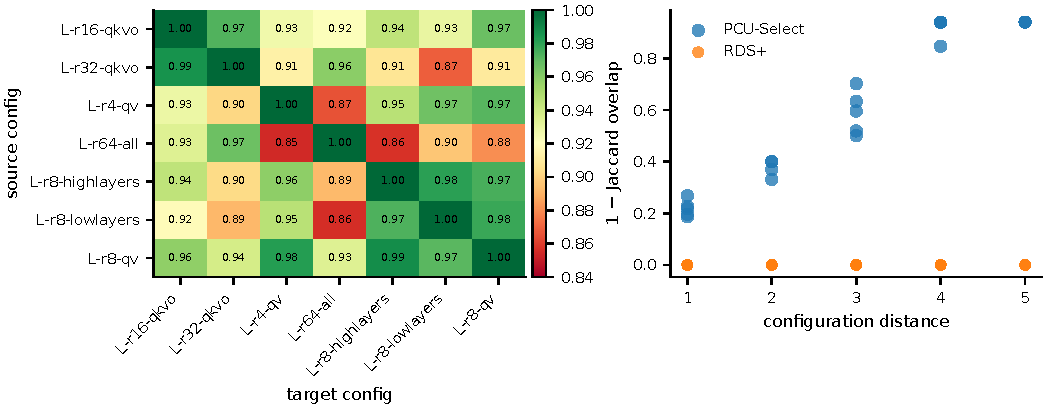
\includegraphics[width=\textwidth]{Figures/fig_config_sensitivity.pdf}
\caption{PCU-Select responds to configuration changes. \emph{Left:} Rows denote
the PEFT used for selection and columns the PEFT used for target training; each
column is normalized by its matched diagonal. The mean normalized off-diagonal
drop is $0.068$. On the unnormalized scale, the matched and mismatched means are
21.25 and 19.79, respectively, a $1.46$-point gap. \emph{Right:} Selection
difference, measured as $1-$Jaccard, versus the heuristic distance
$|\log_2 r_i-\log_2 r_j|+\mathbb{I}[\text{placement differs}]
+\mathbb{I}[\text{module set differs}]$. Across the 21 unordered pairs of seven
LoRA configurations, the descriptive Spearman correlation is $\rho=0.969$;
leave-one-configuration-out values span $[0.947,0.972]$. RDS+ lies at zero
because, for a fixed task, its ranking is PEFT-independent.}
\label{fig:config-sensitivity}
\end{figure*}

\paragraph{Unseen-configuration transfer.}
Table~\ref{tab:ood-levels} reports the values plotted in Figure~3 of the main paper.
Near-support targets transfer zero-shot.
Calibration closes most of the gap for far same-family targets and LN Tuning.
For Prefix/P-Tuning, the point estimate falls from 6.97 to 1.99 but leaves a
larger residual gap than for L1 or LN Tuning. The 0.18 change from Cal-200 to
Cal-500 is descriptive rather than evidence of a reliable difference between
the two label budgets.

\begin{table*}[t]
\centering
\small
\setlength{\tabcolsep}{4pt}
\begin{tabular}{lllrrr}
\toprule
Tier & Targets & Ref. & Zero-shot & Cal-200 & Cal-500 \\
\midrule
L0 & L-r32-qkvo, AD-b16 & LESS & 0.34$\pm$0.41 & -- & -- \\
L1 & L-r64-all, AD-b256, L-r8-highlayers & LESS & 2.08$\pm$0.44 & 0.91$\pm$0.29 & 0.30$\pm$0.36 \\
L2-BF & BF & LESS & 4.08$\pm$0.70 & 0.65$\pm$0.26 & 0.23$\pm$0.42 \\
L2-Prompt & PRE-l16, PT-l32 & RDS+ & 6.97$\pm$0.34 & -- & -- \\
\bottomrule
\end{tabular}
\caption{Performance drop from the named reference across GSM8K, HumanEval, and MMLU (reference minus PCU-Select; paired mean$\pm$sample SD over three target-training seeds). Lower is better; zero denotes parity. L0 uses zero-shot only. Calibration reduces far same-family and BitFit drops. Prefix/P-Tuning lack compatible labels.}
\label{tab:ood-levels}
\end{table*}


\subsection{Baseline Specifications}
\label{sec:appendix-baselines}

The three named baselines span two relevant axes: whether selection uses
gradients and whether its scoring signal depends on the target PEFT. They are
not single-factor ablations; the component ablations above isolate individual
PCU-Select design choices. We specify each implementation below so that the
comparison is auditable.

\paragraph{RDS+ (representation similarity).}
RDS+ operates on the 768-dimensional joint semantic embedding
$e_x^{\text{joint}}$ produced by the frozen sentence encoder. This is the
semantic component of PCU-Select's sample representation $z_x$. RDS+ neither
trains the encoder nor uses features learned by the PCU-Select scorer.

RDS+ first standardizes every pool embedding per feature. It forms the query by
averaging the 32 task-sketch embeddings and applies the same pool statistics. It
then $L_2$-normalizes the pool and query vectors and ranks candidates by cosine
similarity.

RDS+ is \emph{task-conditioned} through the sketch query but
\emph{PEFT-agnostic}: its ranking does not depend on the target configuration.
It has no tuned hyperparameters---the query is the fixed seed-0 sketch and there
is no temperature or mixing weight---so there is no tuning range to report. The
``+'' denotes the per-feature standardization applied before cosine, relative to
a plain embedding-nearest-neighbor selector.

\paragraph{Influence (shared-datastore gradient similarity).}
The Influence baseline builds one shared projected-gradient datastore from the
base model's intervention-site activations. It uses the JL projection and $L_2$
normalization specified in the reproducibility notes. Each candidate carries
signatures $g_x^\omega$ at the 24 sites. The task query $g_t^\omega$ pools and
renormalizes the sketch gradient at each site. Influence scores each candidate
with the plain cosine $\sum_{\omega}\cos(g_x^\omega, g_t^\omega)$ and applies
global top-$k$ without site weighting. Its PEFT-agnostic gradient source makes
the ranking independent of the target configuration. Influence therefore
provides a PEFT-agnostic shared-gradient reference; its comparison with
PCU-Select does not by itself isolate the effect of PEFT conditioning.

\paragraph{LESS (per-PEFT gradient influence).}
LESS is a per-configuration reimplementation of gradient-influence selection
following LESS~\cite{xia2024less}. It applies four steps to each target PEFT.
First, it warms up the target adapter for $200$ steps to obtain the optimization
state. Second, it extracts Adam-preconditioned gradients over the adapter's own
trainable parameters at each checkpoint. Third, it projects the gradients into a
target-specific low-dimensional datastore. Finally, it ranks candidates by their
projected-gradient influence on the 32-example task sketch and averages across
warmup checkpoints.

The first three steps build the datastore over the target adapter's own
trainable parameters. The datastore is therefore PEFT-specific but
task-independent. LESS constructs it once per PEFT and reuses it for every task
sketch. Only the final projected-gradient scoring step is task-specific.

It costs about $0.30$ GPU-hours per task, so $1.20$ covers all four task sketches
for one configuration. The per-target cost of a PEFT configuration is therefore
$62.0$ (datastore) $+\,1.20$ (four per-task rankings) $=63.2$ GPU-hours, already
spanning the full four-task evaluation; the five-PEFT registry cost is
$5\times63.2=316.0$. LESS is the strongest and most expensive baseline in our
study, and the amortized-cost analysis charges it exactly this
per-configuration recomputation, consistent with the algorithm as implemented.

\paragraph{Baseline configuration and tuning.}
Random has no hyperparameters. RDS+ uses the fixed representation-similarity
rule above with the shared $32$-example sketch as its only task input. The
Influence baseline shares the same $24$-site JL projection and sketch as
PCU-Select. We fix every baseline's hyperparameters before test-metric
evaluation.
